% Options for packages loaded elsewhere
\PassOptionsToPackage{unicode}{hyperref}
\PassOptionsToPackage{hyphens}{url}
\PassOptionsToPackage{dvipsnames,svgnames,x11names}{xcolor}
%
\documentclass[
  letterpaper,
  DIV=11,
  numbers=noendperiod]{scrartcl}

\usepackage{amsmath,amssymb}
\usepackage{iftex}
\ifPDFTeX
  \usepackage[T1]{fontenc}
  \usepackage[utf8]{inputenc}
  \usepackage{textcomp} % provide euro and other symbols
\else % if luatex or xetex
  \usepackage{unicode-math}
  \defaultfontfeatures{Scale=MatchLowercase}
  \defaultfontfeatures[\rmfamily]{Ligatures=TeX,Scale=1}
\fi
\usepackage{lmodern}
\ifPDFTeX\else  
    % xetex/luatex font selection
\fi
% Use upquote if available, for straight quotes in verbatim environments
\IfFileExists{upquote.sty}{\usepackage{upquote}}{}
\IfFileExists{microtype.sty}{% use microtype if available
  \usepackage[]{microtype}
  \UseMicrotypeSet[protrusion]{basicmath} % disable protrusion for tt fonts
}{}
\makeatletter
\@ifundefined{KOMAClassName}{% if non-KOMA class
  \IfFileExists{parskip.sty}{%
    \usepackage{parskip}
  }{% else
    \setlength{\parindent}{0pt}
    \setlength{\parskip}{6pt plus 2pt minus 1pt}}
}{% if KOMA class
  \KOMAoptions{parskip=half}}
\makeatother
\usepackage{xcolor}
\setlength{\emergencystretch}{3em} % prevent overfull lines
\setcounter{secnumdepth}{5}
% Make \paragraph and \subparagraph free-standing
\makeatletter
\ifx\paragraph\undefined\else
  \let\oldparagraph\paragraph
  \renewcommand{\paragraph}{
    \@ifstar
      \xxxParagraphStar
      \xxxParagraphNoStar
  }
  \newcommand{\xxxParagraphStar}[1]{\oldparagraph*{#1}\mbox{}}
  \newcommand{\xxxParagraphNoStar}[1]{\oldparagraph{#1}\mbox{}}
\fi
\ifx\subparagraph\undefined\else
  \let\oldsubparagraph\subparagraph
  \renewcommand{\subparagraph}{
    \@ifstar
      \xxxSubParagraphStar
      \xxxSubParagraphNoStar
  }
  \newcommand{\xxxSubParagraphStar}[1]{\oldsubparagraph*{#1}\mbox{}}
  \newcommand{\xxxSubParagraphNoStar}[1]{\oldsubparagraph{#1}\mbox{}}
\fi
\makeatother


\providecommand{\tightlist}{%
  \setlength{\itemsep}{0pt}\setlength{\parskip}{0pt}}\usepackage{longtable,booktabs,array}
\usepackage{calc} % for calculating minipage widths
% Correct order of tables after \paragraph or \subparagraph
\usepackage{etoolbox}
\makeatletter
\patchcmd\longtable{\par}{\if@noskipsec\mbox{}\fi\par}{}{}
\makeatother
% Allow footnotes in longtable head/foot
\IfFileExists{footnotehyper.sty}{\usepackage{footnotehyper}}{\usepackage{footnote}}
\makesavenoteenv{longtable}
\usepackage{graphicx}
\makeatletter
\newsavebox\pandoc@box
\newcommand*\pandocbounded[1]{% scales image to fit in text height/width
  \sbox\pandoc@box{#1}%
  \Gscale@div\@tempa{\textheight}{\dimexpr\ht\pandoc@box+\dp\pandoc@box\relax}%
  \Gscale@div\@tempb{\linewidth}{\wd\pandoc@box}%
  \ifdim\@tempb\p@<\@tempa\p@\let\@tempa\@tempb\fi% select the smaller of both
  \ifdim\@tempa\p@<\p@\scalebox{\@tempa}{\usebox\pandoc@box}%
  \else\usebox{\pandoc@box}%
  \fi%
}
% Set default figure placement to htbp
\def\fps@figure{htbp}
\makeatother

\KOMAoption{captions}{tableheading}
\makeatletter
\@ifpackageloaded{caption}{}{\usepackage{caption}}
\AtBeginDocument{%
\ifdefined\contentsname
  \renewcommand*\contentsname{Table of contents}
\else
  \newcommand\contentsname{Table of contents}
\fi
\ifdefined\listfigurename
  \renewcommand*\listfigurename{List of Figures}
\else
  \newcommand\listfigurename{List of Figures}
\fi
\ifdefined\listtablename
  \renewcommand*\listtablename{List of Tables}
\else
  \newcommand\listtablename{List of Tables}
\fi
\ifdefined\figurename
  \renewcommand*\figurename{Figure}
\else
  \newcommand\figurename{Figure}
\fi
\ifdefined\tablename
  \renewcommand*\tablename{Table}
\else
  \newcommand\tablename{Table}
\fi
}
\@ifpackageloaded{float}{}{\usepackage{float}}
\floatstyle{ruled}
\@ifundefined{c@chapter}{\newfloat{codelisting}{h}{lop}}{\newfloat{codelisting}{h}{lop}[chapter]}
\floatname{codelisting}{Listing}
\newcommand*\listoflistings{\listof{codelisting}{List of Listings}}
\makeatother
\makeatletter
\makeatother
\makeatletter
\@ifpackageloaded{caption}{}{\usepackage{caption}}
\@ifpackageloaded{subcaption}{}{\usepackage{subcaption}}
\makeatother

\usepackage{bookmark}

\IfFileExists{xurl.sty}{\usepackage{xurl}}{} % add URL line breaks if available
\urlstyle{same} % disable monospaced font for URLs
\hypersetup{
  pdftitle={Analysis of class surveys},
  pdfauthor={Justin Zhou,Ella Yang,Lucy Cao,Cecilia Jiang,Janice Jiang,Wendy Zhu},
  colorlinks=true,
  linkcolor={blue},
  filecolor={Maroon},
  citecolor={Blue},
  urlcolor={Blue},
  pdfcreator={LaTeX via pandoc}}


\title{Analysis of class surveys}
\usepackage{etoolbox}
\makeatletter
\providecommand{\subtitle}[1]{% add subtitle to \maketitle
  \apptocmd{\@title}{\par {\large #1 \par}}{}{}
}
\makeatother
\subtitle{Part 1: Is self-reported statistics proficiency associated
with the number of PSTAT courses completed?}
\author{Justin Zhou,Ella Yang,Lucy Cao,Cecilia Jiang,Janice Jiang,Wendy
Zhu}
\date{2025-10-19}

\begin{document}
\maketitle

\renewcommand*\contentsname{Table of contents}
{
\hypersetup{linkcolor=}
\setcounter{tocdepth}{3}
\tableofcontents
}

\section{Executive summary}\label{executive-summary}

We analyzed anonymized intake-survey responses from two sections to
answer one question: \textbf{Is self-reported statistics proficiency
associated with the number of PSTAT courses completed?} Using
descriptive plots and a one-way ANOVA with Tukey's post-hoc test
(implemented in \texttt{Question\_1.Rmd}), we find evidence of a
statistically significant association: respondents reporting higher
statistics proficiency have, on average, completed more PSTAT courses.
Because the responses are a \textbf{sample} of offered-seat students, we
emphasize clear visuals and center-focused summaries appropriate for
modest (n).

\section{Data description}\label{data-description}

\begin{itemize}
\tightlist
\item
  \textbf{How obtained.} Google Forms intake survey; exported and shared
  as two section files with identifiers removed plus a metadata file.\\
\item
  \textbf{Sample.} Respondents from two course sections; treated as a
  \textbf{sample} from all offered-seat students (not necessarily a
  census).\\
\item
  \textbf{Measurements.} Demographics; self-assessed
  \textbf{proficiency} and \textbf{comfort} (Likert 1--5); indicators
  for prior coursework; and project preferences. For Q1, we use
  \texttt{stat.prof} (statistics proficiency; ordered beginner →
  intermediate → advanced) and \texttt{pstat\_courses\_total} (sum of
  PSTAT course indicators per student).
\end{itemize}

\section{Question of interest}\label{question-of-interest}

\begin{enumerate}
\def\labelenumi{\arabic{enumi}.}
\tightlist
\item
  \textbf{Q1.} Does self-reported statistics proficiency relate to the
  number of PSTAT courses completed?
\end{enumerate}

\section{Findings (Q1)}\label{findings-q1}

\textbf{Question.} Is self-reported statistics proficiency associated
with the number of PSTAT courses completed?

\textbf{What we did.} We summarized the distribution of proficiency
levels (Beginner, Intermediate, Advanced) and compared total PSTAT
coursework across groups using descriptive plots (composition chart,
boxplot, and mean ± SD bar chart with a trend view). We then ran a
one-way ANOVA and Tukey's HSD post-hoc comparisons using the code in
\texttt{results/Question\_1.Rmd}.

\subsection{Proficiency composition}\label{proficiency-composition}

\begin{figure}[H]

{\centering \pandocbounded{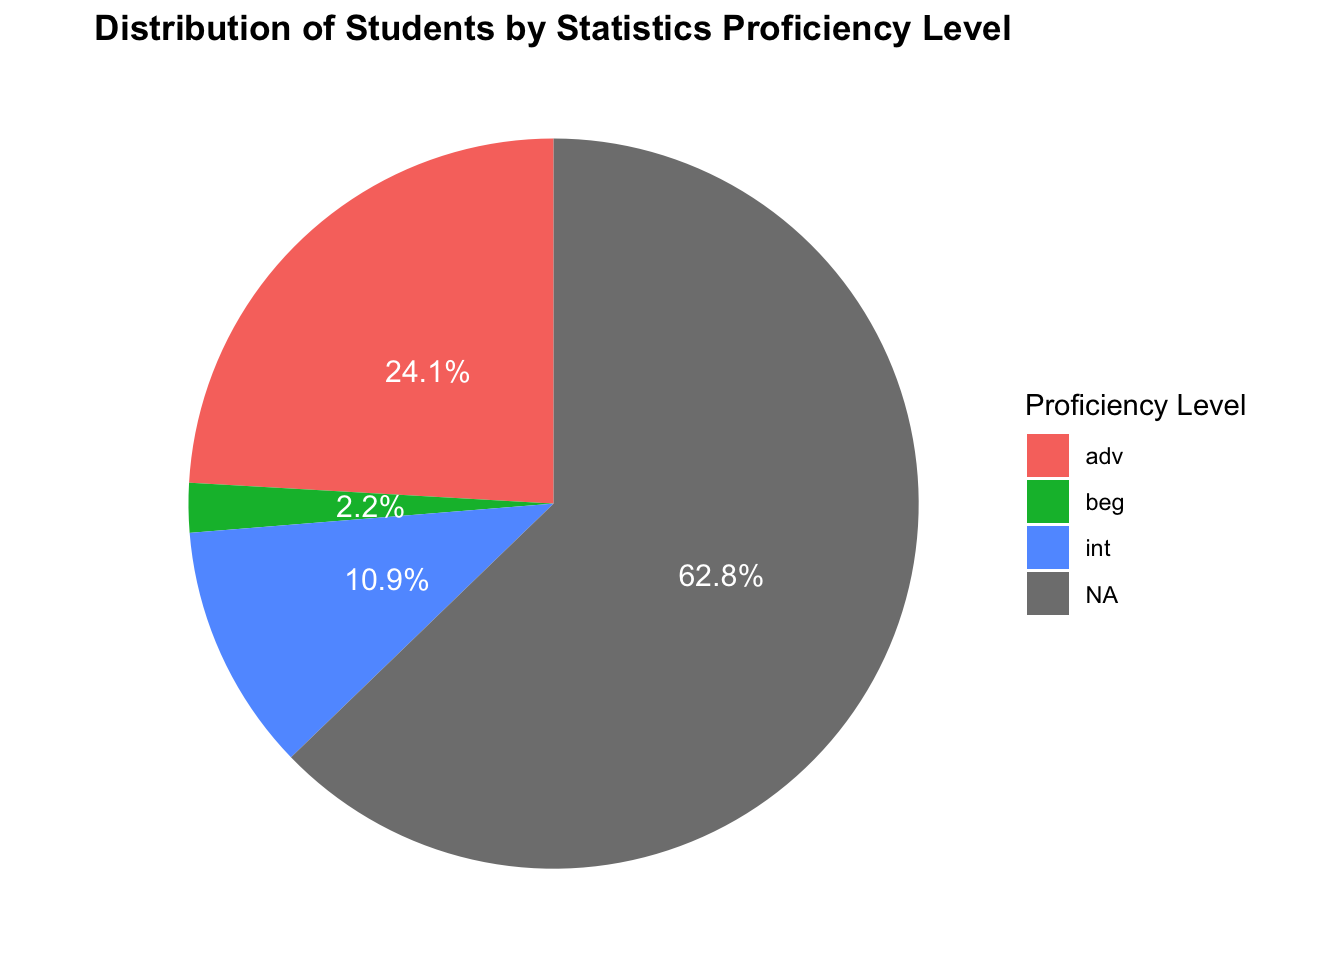
\includegraphics[keepaspectratio]{Untitled/unnamed-chunk-3-1.png}}

}

\caption{Distribution of Students by Statistics Proficiency Level}

\end{figure}%

Most respondents did not record a proficiency level (NA is the largest
slice). Among those who did, Advanced is more common than Intermediate,
and Beginner is the smallest group. This matters for two reasons: (1)
our comparisons are essentially between a larger Advanced group and
smaller Intermediate/Beginner groups, and (2) inferential tests should
exclude the NA category since it is missing-by-design.

\subsection{PSTAT courses by proficiency
(boxplot)}\label{pstat-courses-by-proficiency-boxplot}

\begin{figure}[H]

{\centering \pandocbounded{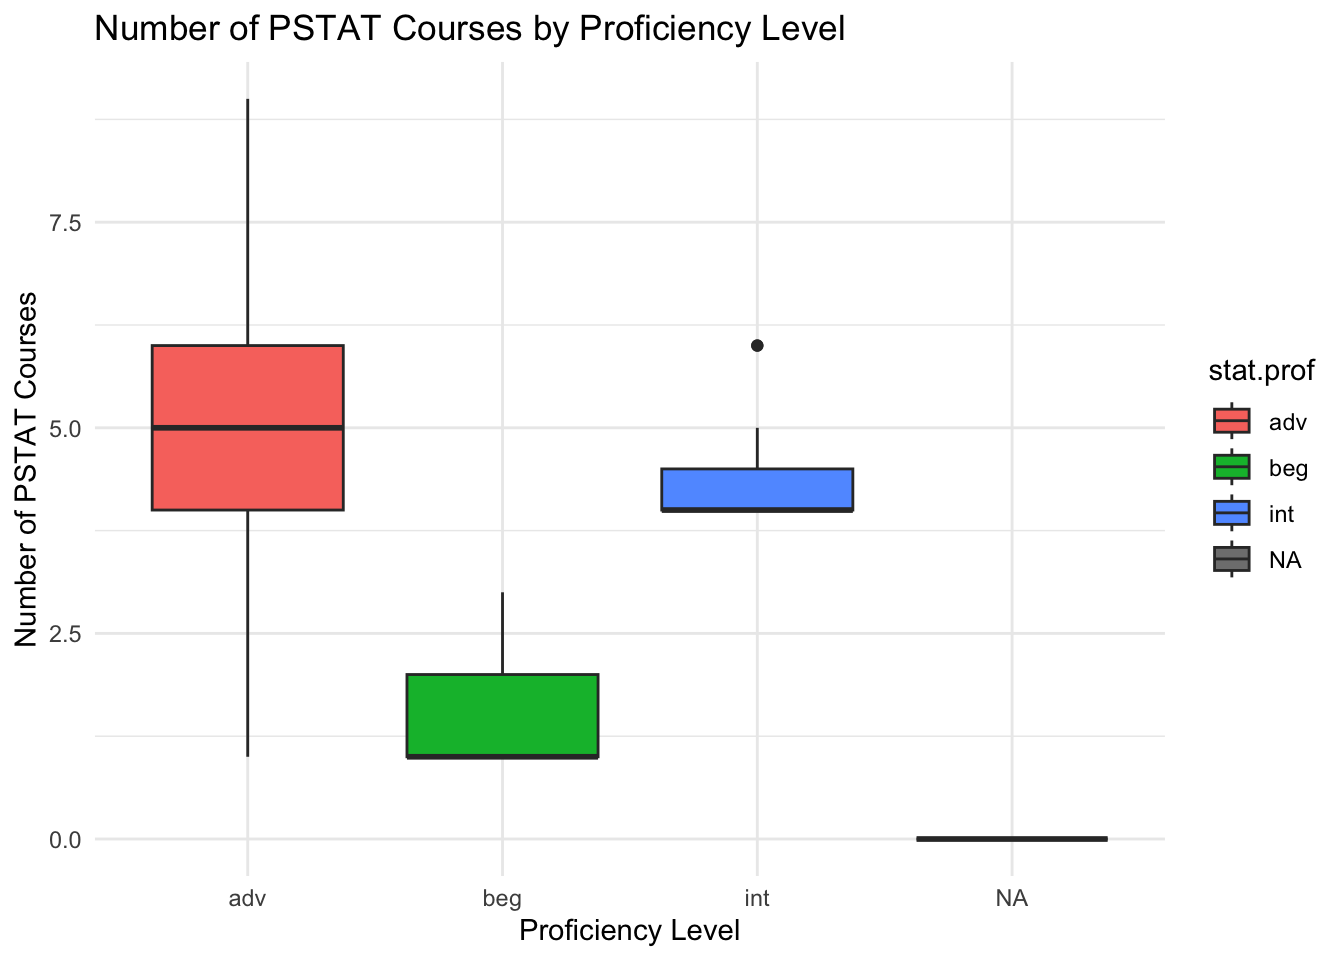
\includegraphics[keepaspectratio]{Untitled/unnamed-chunk-4-1.png}}

}

\caption{Number of PSTAT Courses by Proficiency Level}

\end{figure}%

The center and spread of completed PSTAT courses shift upward from
Beginner -\textgreater{} Intermediate -\textgreater{} Advanced.
Beginners cluster at the low end; Intermediate has a higher median with
modest spread; Advanced shows both a higher median and a longer right
tail (some students have many courses). The NA group appears at zero
because proficiency was not reported; we do not use NA in tests.
Overlapping IQRs are limited, which is consistent with a real difference
in central tendency.

\subsection{Average PSTAT courses (mean ±
SD)}\label{average-pstat-courses-mean-sd}

\pandocbounded{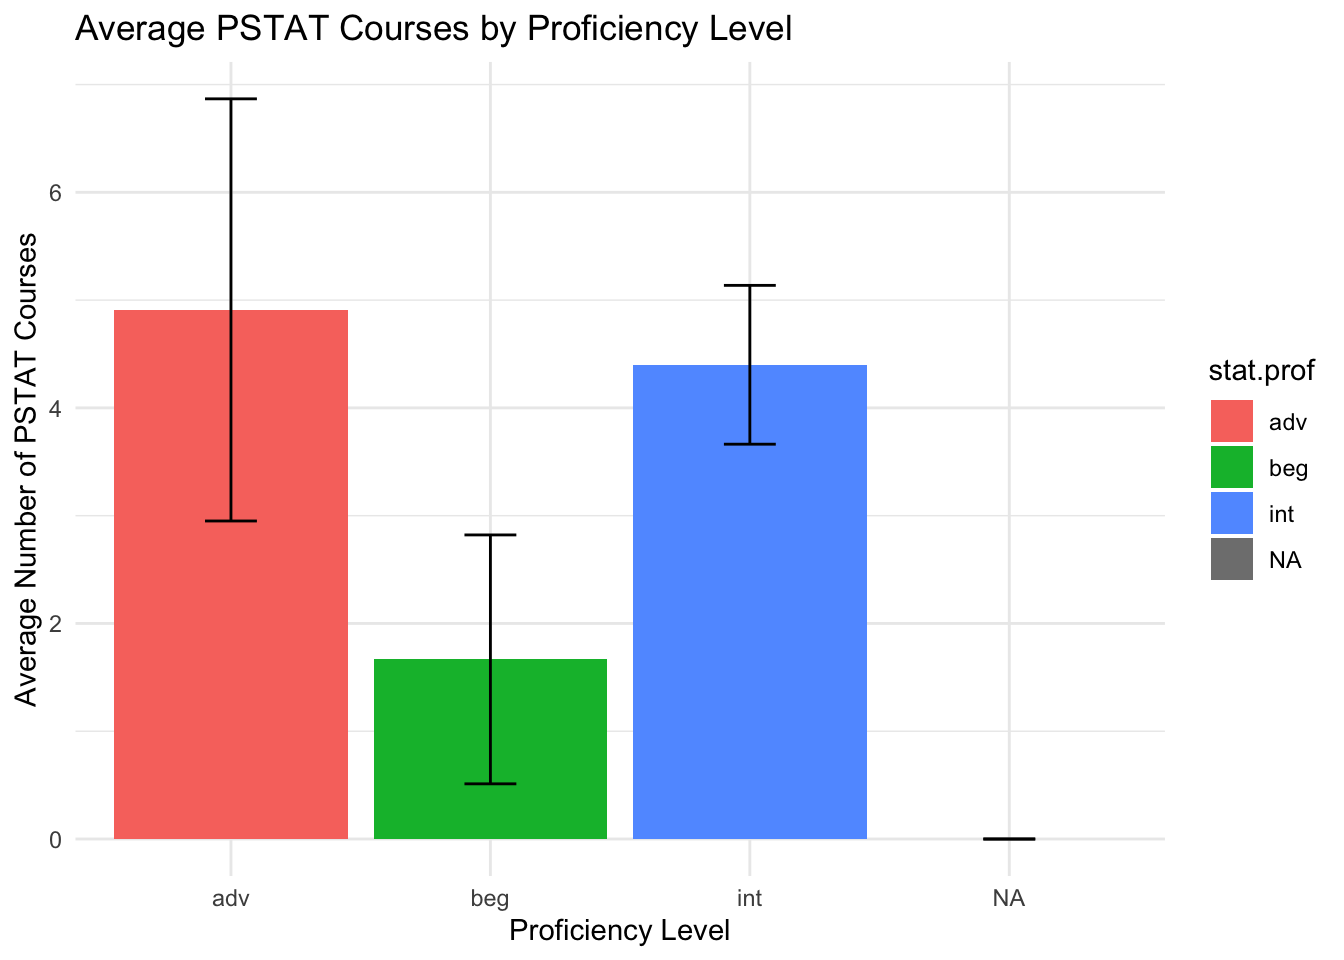
\includegraphics[keepaspectratio]{Untitled/unnamed-chunk-5-1.png}}
Group means increase with proficiency: Beginners average the fewest
PSTAT courses, Intermediate is higher, and Advanced is highest. Error
bars (\$\pm\$1 SD) overlap somewhat between Intermediate and Advanced,
suggesting those two groups are similar on average. This aligns with the
Tukey HSD results: both Intermediate and Advanced differ from Beginners,
while Intermediate and Advanced are not statistically different from
each other.

\subsection{Average PSTAT courses
(trend)}\label{average-pstat-courses-trend}

\begin{figure}[H]

{\centering \pandocbounded{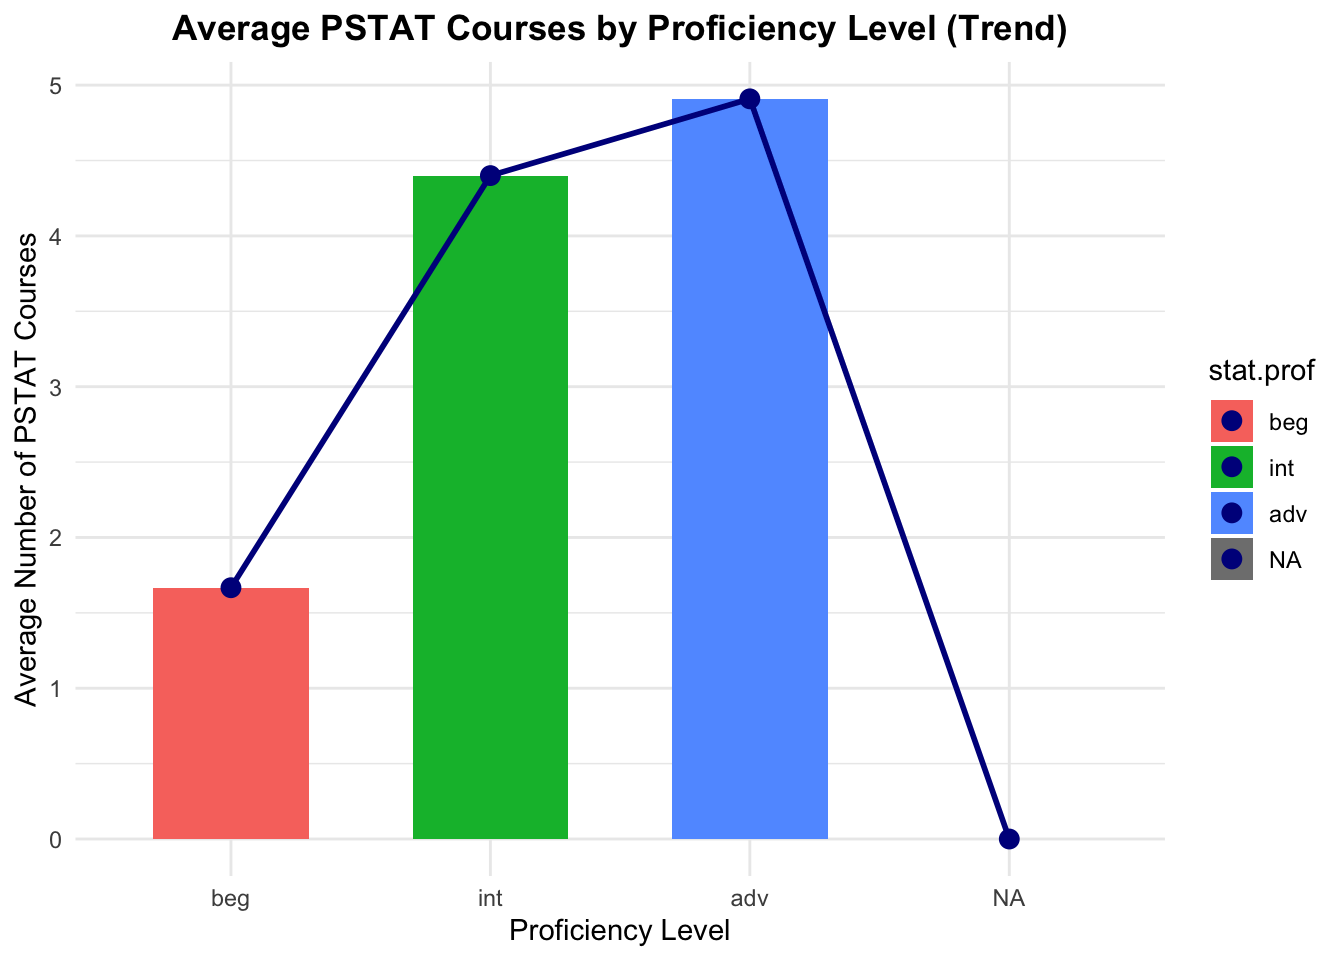
\includegraphics[keepaspectratio]{Untitled/unnamed-chunk-6-1.png}}

}

\caption{Average PSTAT Courses by Proficiency Level (Trend)}

\end{figure}%

The trend line provides a compact view of the monotone relationship:
more completed PSTAT courses are associated with higher self--reported
proficiency. The drop to zero at NA reflects missing proficiency rather
than a true value and should not be interpreted substantively. Overall,
the trend corroborates the boxplot and mean \(\pm\) SD views.

\begin{center}\rule{0.5\linewidth}{0.5pt}\end{center}

\subsection{Inferential check (supports the
visuals)}\label{inferential-check-supports-the-visuals}

\begin{itemize}
\tightlist
\item
  \textbf{One-way ANOVA:} p = 0.008 (alpha = 0.05) -\textgreater{} mean
  PSTAT courses differ across proficiency groups.
\item
  \textbf{Tukey's HSD pairwise comparisons:}

  \begin{itemize}
  \tightlist
  \item
    Advanced vs Beginner: p = 0.0062 (significant)
  \item
    Intermediate vs Beginner: p = 0.033 (significant)
  \item
    Intermediate vs Advanced: p = 0.59 (not significant)
  \end{itemize}
\end{itemize}

\textbf{Conclusion from tests:} The main differences are between
\textbf{Beginners} and the other two groups; \textbf{Intermediate} and
\textbf{Advanced} are not statistically different in this sample.

\begin{center}\rule{0.5\linewidth}{0.5pt}\end{center}

\subsection{Important decisions (for
reproducibility)}\label{important-decisions-for-reproducibility}

\begin{itemize}
\tightlist
\item
  Constructed \texttt{pstat\_courses\_total} by summing the binary PSTAT
  course indicators per student.\\
\item
  Treated \texttt{stat.prof} as an \textbf{ordered} factor with levels
  \texttt{beg\ \textless{}\ int\ \textless{}\ adv}.\\
\item
  \textbf{NA} in \texttt{stat.prof} are shown in composition plots but
  excluded from ANOVA/Tukey.\\
\item
  Emphasized \textbf{medians/IQRs} (boxplot) alongside means ± SD to
  avoid over-interpreting tails for modest sample sizes.
\end{itemize}

\subsection{Interpretation and scope}\label{interpretation-and-scope}

Within this sample of students offered a seat, \textbf{greater PSTAT
coursework is associated with higher self-reported statistics
proficiency}, especially when comparing \textbf{Beginners} to
\textbf{Intermediate/Advanced}. Because this is a respondent sample with
some item nonresponse, we treat results as \textbf{descriptive evidence}
rather than a population claim.

\textbf{Possible extensions.} Report group counts and medians in the
text; check robustness with a non-parametric Kruskal--Wallis test;
examine whether particular PSTAT sequences (e.g., 120/122/126) align
most with higher self-ratings.

\section{Findings (Q2)}\label{findings-q2}

\textbf{Question.}

How will the number of Computer Science courses that a student takes
affects the students' programming proficiency?

\textbf{Overview} For this question, we investigate on whether the
number of computer science (CS) courses a student has taken is
associated with their self-reported programming proficiency level. The
goal is to determine if greater exposure to CS coursework corresponds to
higher programming skill levels, as measured by students' proficiency
categories (beginner, intermediate, advanced) in the survey dataset.

\textbf{Data and Methodology} We derived the variable cs\_total,
representing the total number of CS courses each student completed, by
summing binary indicators for each course. In addition to core CS
courses (e.g., CS 9, CS 16, CS 130), we also included PSTAT 100, 131,
and 134, since these courses require programming in R and involve data
manipulation, which contributes to programming experience. Programming
proficiency was encoded numerically (1 = Beginner, 2 = Intermediate, 3 =
Advanced) to facilitate regression and visualization. We then ran a
simple linear regression model to evaluate the relationship between
cs\_total and prof.

\subsection{Proficiency composition}\label{proficiency-composition-1}

\pandocbounded{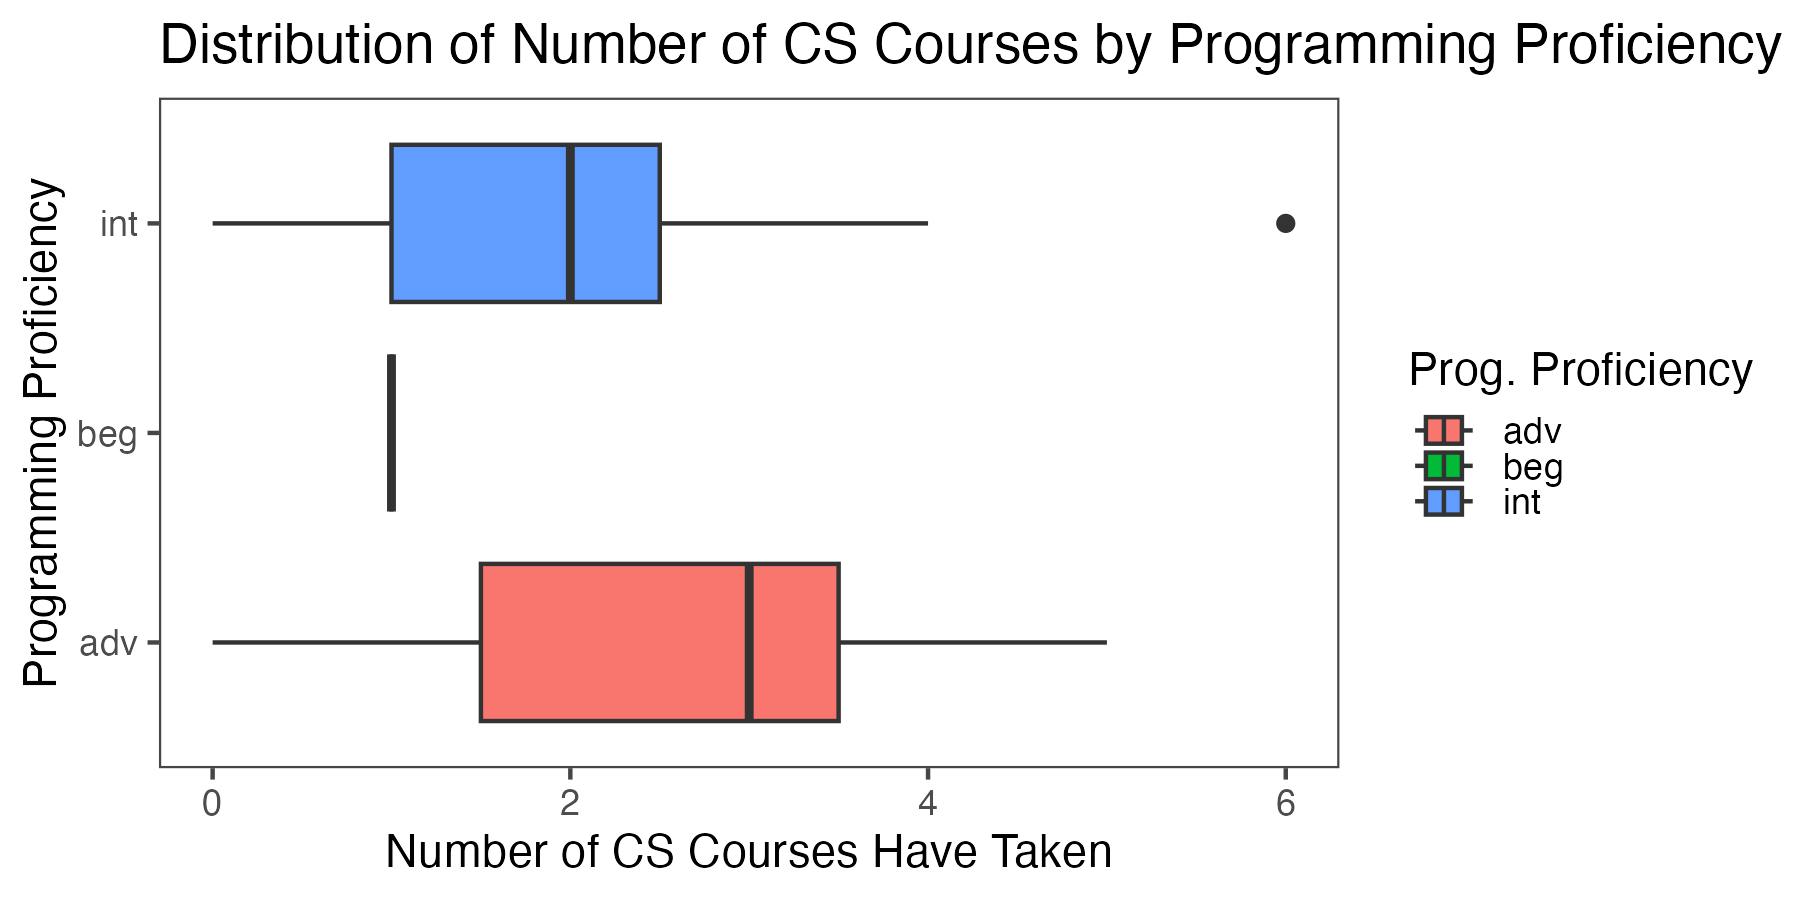
\includegraphics[keepaspectratio]{Untitled/Distribution of Number of CS Courses by Programming Proficiency.png}}
\textbf{Description} This boxplot displays the distribution of the total
number of CS courses taken for each programming proficiency group
(beginner, intermediate, advanced). The x-axis represents the number of
CS courses taken, while the y-axis categorizes students by their
self-reported proficiency.

\textbf{Interpretation:} From the graph, we can observe that:

\textbf{Advanced students (red)} tend to have taken more CS courses on
average than intermediate or beginner students. Their interquartile
range is higher, and their median is around 2--3 courses.

\textbf{Intermediate students (blue)} show a slightly lower median but
also a wider spread, ranging from 1 to 5 courses, with a few outliers
who have taken 6 or more.

\textbf{Beginners (green)} have taken very few or no CS courses, with
their distribution concentrated near 0--1.

Overall, this pattern \textbf{supports the hypothesis that taking more
CS courses generally corresponds to higher programming proficiency.}
However, the overlap between intermediate and advanced groups suggests
that coursework alone does not fully determine skill level---experience
outside formal classes might also influence proficiency.

\pandocbounded{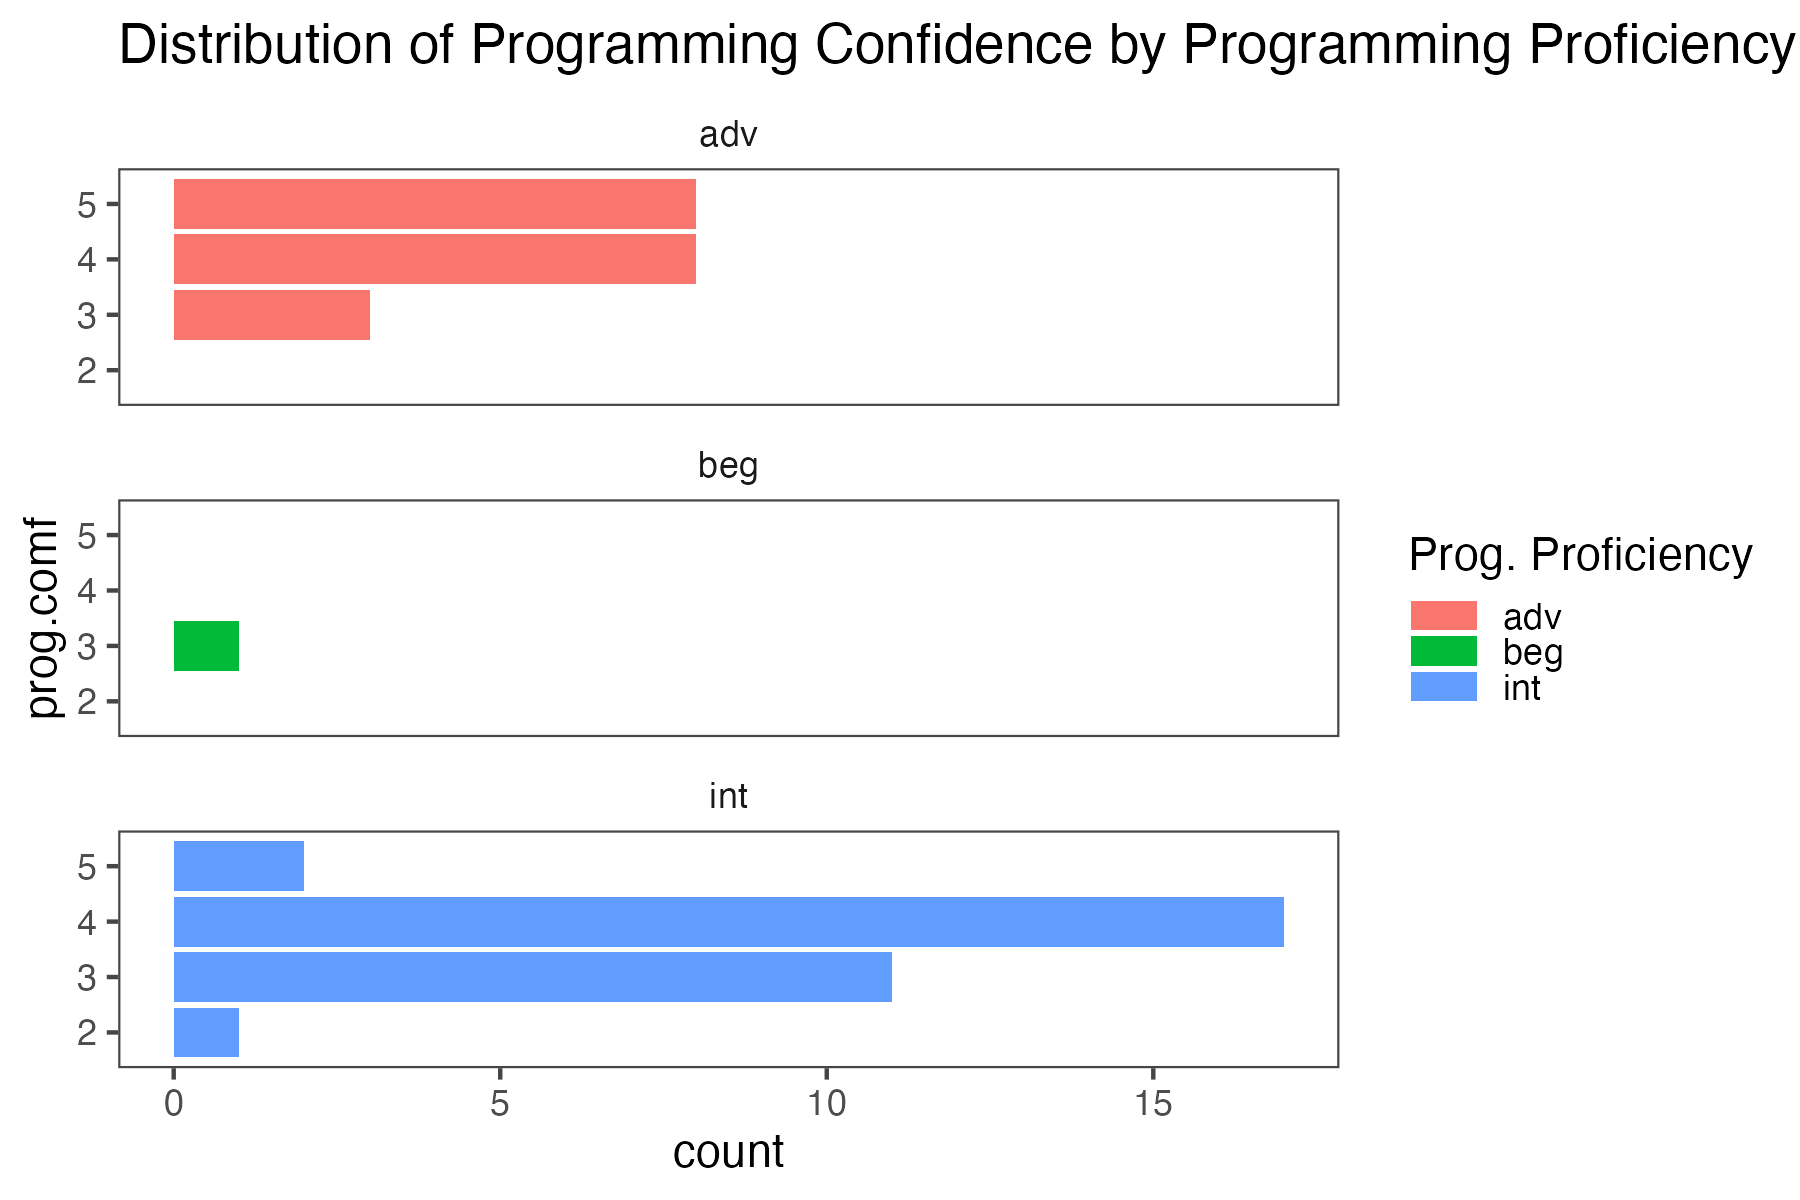
\includegraphics[keepaspectratio]{Untitled/Distribution of Programming Confidence by Programming Proficiency.png}}
\textbf{Description:} This bar chart shows how students' self-reported
confidence levels (1--5 scale) vary across different proficiency groups.
Each bar indicates the count of students who selected a given confidence
rating.

\textbf{Interpretation:} Students in the advanced group mostly report
high confidence levels, typically 4 or 5, indicating consistency between
their proficiency and self-assessment.

The intermediate group also shows a large cluster of high confidence
scores (mostly 3--5), which suggests that many intermediate-level
students also very comfortable with programming.

The beginner group is small, but its few members report lower confidence
levels, typically 2--3, as expected.

\textbf{Overall Analysis:} The visualization shows that programming
confidence generally increases with proficiency, but the relationship is
not perfectly linear.

Advanced students show consistently high confidence, as expected.

Intermediate students' confidence overlaps considerably with the
advanced group, indicating subjectivity in self-perceived skill levels.

The variation also highlights that confidence does not always correspond
directly to technical ability---students' previous experiences (e.g.,
PSTAT courses, self-study, or non-CS exposure) may also shape how
confident they feel when coding.

\pandocbounded{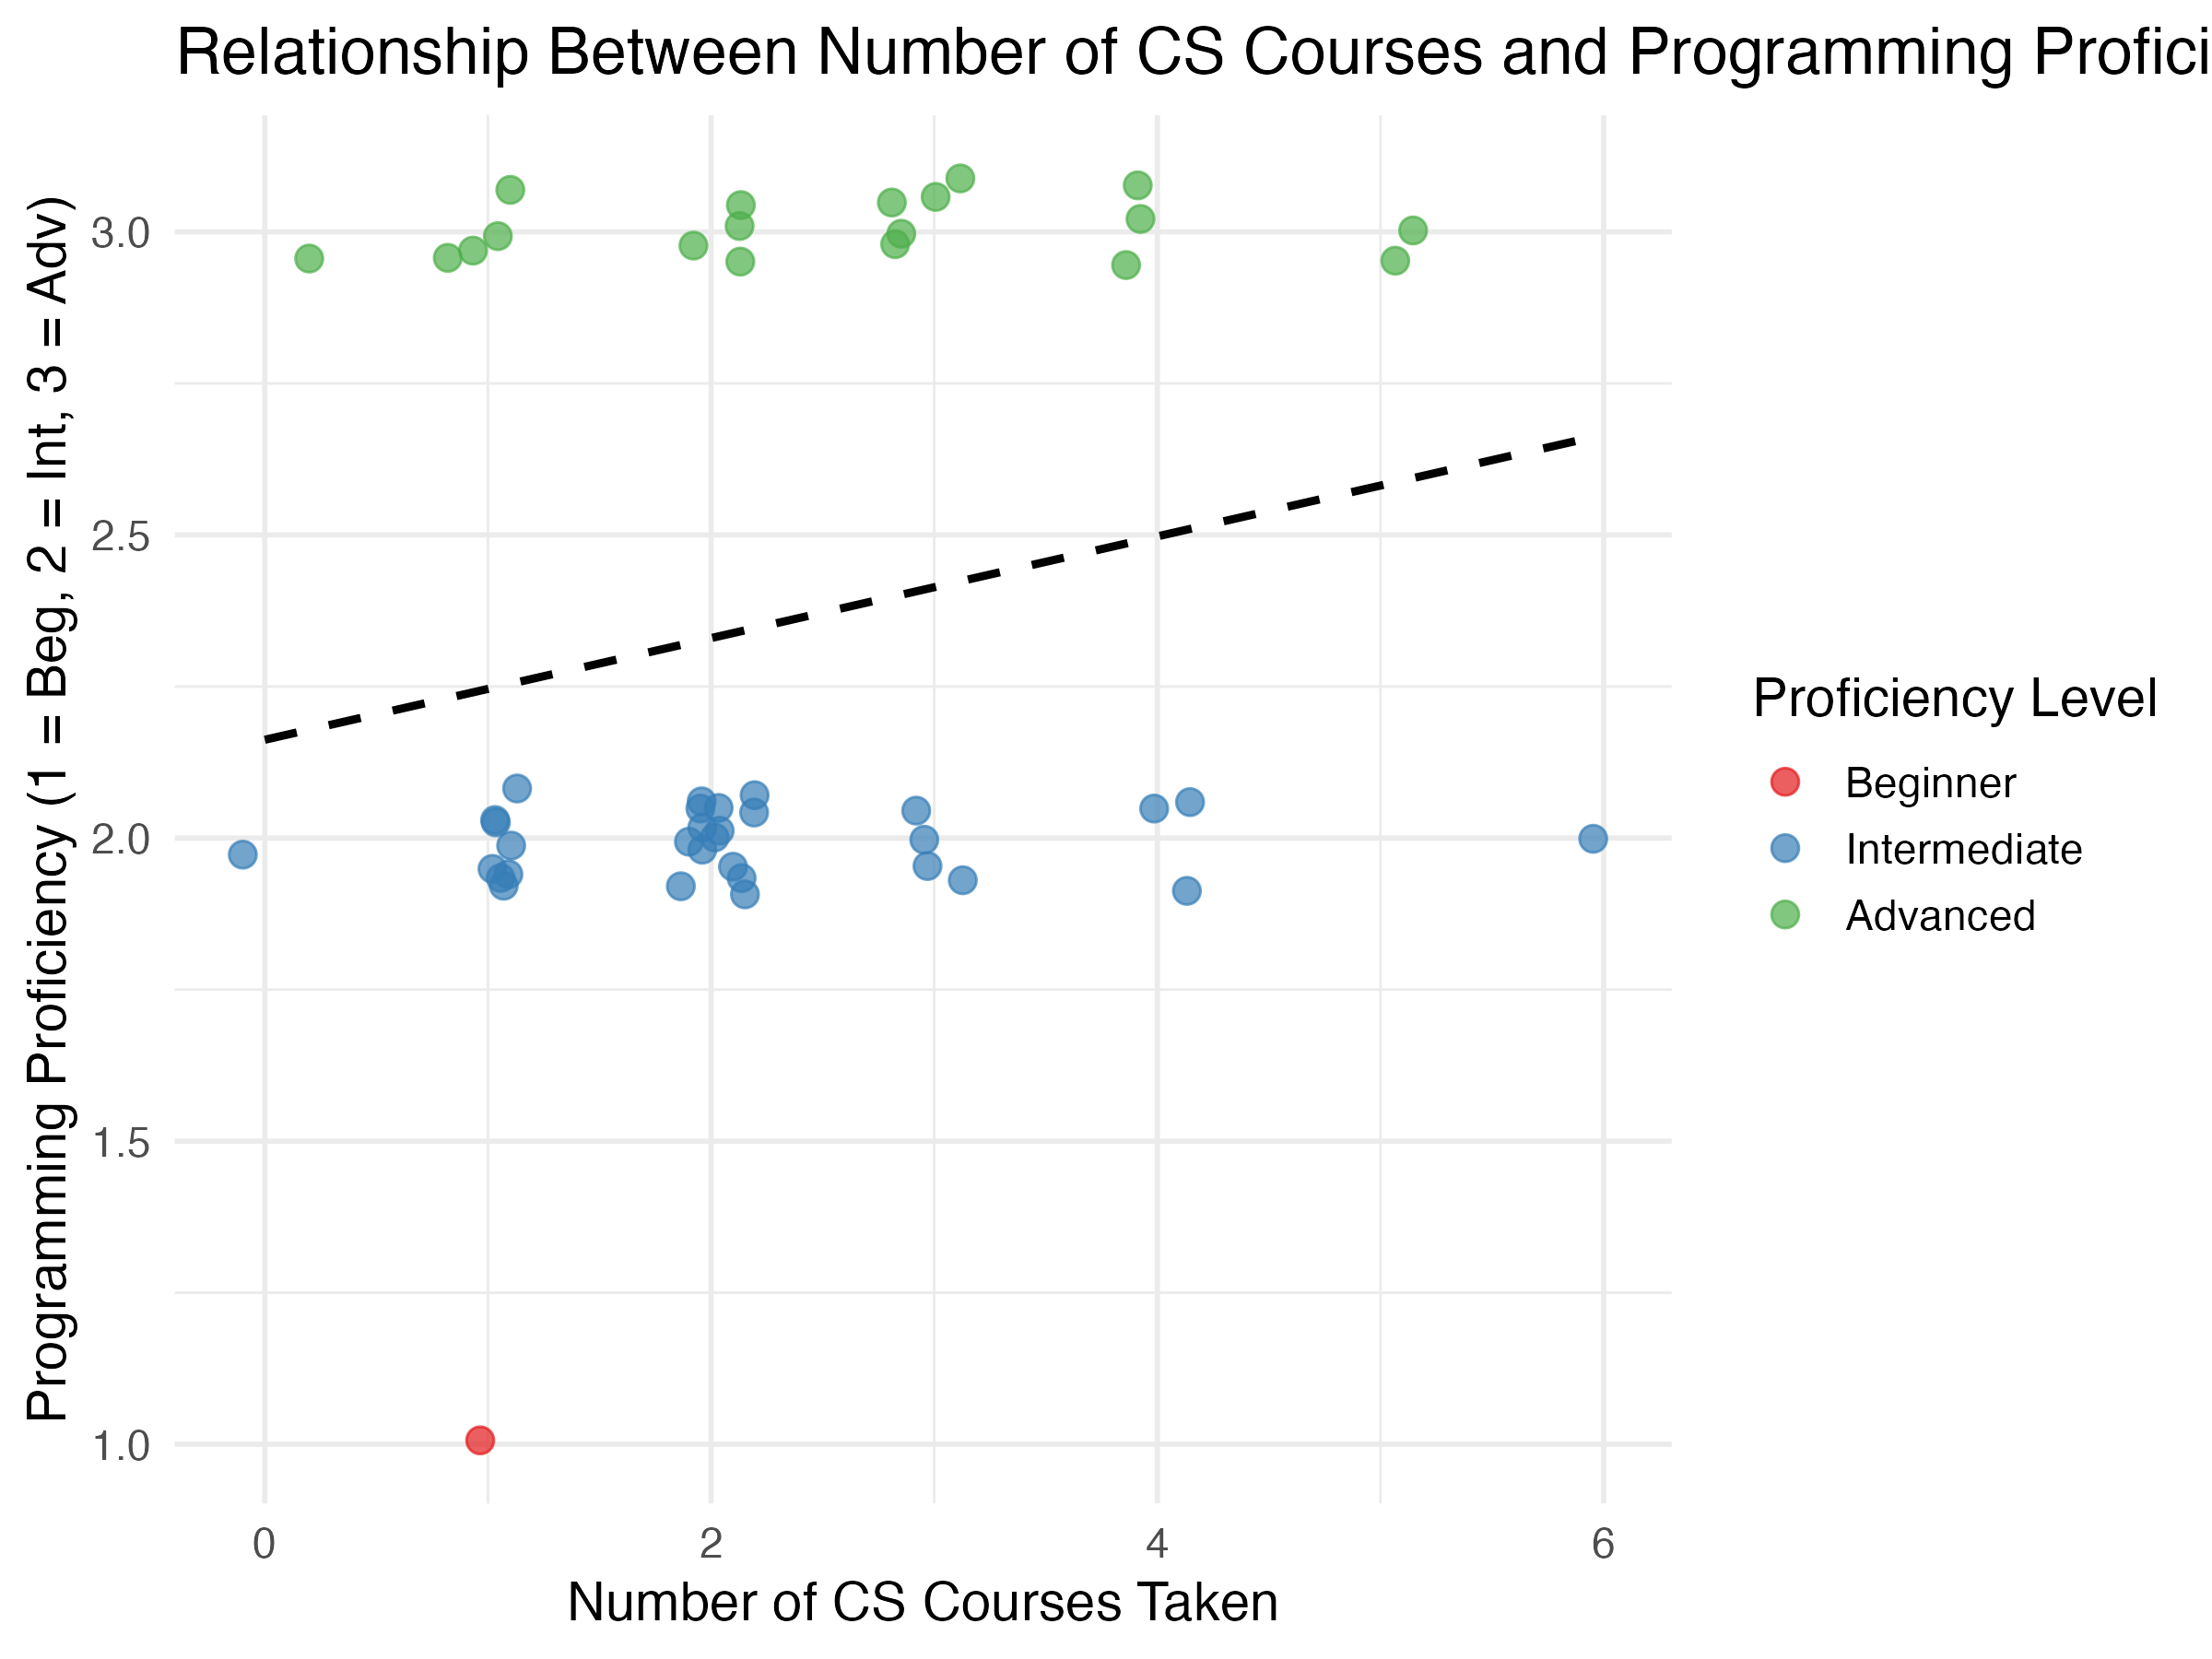
\includegraphics[keepaspectratio]{Untitled/question_2_plot.png}}
\textbf{Description:} This scatterplot displays the relationship between
the number of CS courses taken (x-axis) and students' self-reported
programming proficiency (y-axis, coded as 1 = Beginner, 2 =
Intermediate, 3 = Advanced). Each dot represents one student,
color-coded by proficiency group---red for beginners, blue for
intermediates, and green for advanced. The black dashed line shows the
fitted linear regression trend from the model: Proficiency=β0 +
β1(Number of CS Courses) + ϵ

\textbf{Interpretation:} The plot shows a positive upward trend,
suggesting that students who have taken more CS courses tend to report
higher programming proficiency levels.

1.Trendline:

The dashed regression line slopes upward, indicating a positive
coefficient for cs\_total.

This means that, on average, each additional CS course is associated
with a higher proficiency score.

2.Group Distribution:

Advanced students (green) cluster toward the upper part of the plot
(proficiency ≈ 3) and typically have taken multiple CS courses, ranging
roughly from 2 to 6.

Intermediate students (blue) form the majority and are spread across the
middle range of CS course counts (1--4). Their distribution is
relatively flat, reflecting that many have moderate experience
regardless of exact course count.

Beginners (red) are few and positioned near the lower left---indicating
both low proficiency and minimal course exposure.

3.Overlap \& Variability:

Although the general trend supports a positive relationship, there is
overlap between intermediate and advanced levels. For instance, some
students with 3--4 CS courses still identify as intermediate, while a
few advanced students have taken only 1--2.

This overlap suggests that while formal coursework contributes strongly
to skill development, other learning pathways (e.g., self-study,
statistics programming, or project experience) can also elevate
proficiency.

\textbf{Conclusion:} This visualization reinforces the finding that
coursework exposure is positively associated with programming
proficiency, but not deterministically so. The modest slope of the
regression line and the visible group overlap imply that programming
ability is multifaceted---it reflects not only classroom experience but
also self-learning, cross-disciplinary training (e.g., PSTAT courses),
and students' personal engagement with coding practice.




\end{document}
